\chapter{Аналитическая часть}

В данной части будут приведены задание к лабораторной работе, необходимые для его выполнения определения, а также описаны используемые для его решения алгоритмы.

\section{Определения}

\textit{Простым графом} $G(V,E)$ называется совокупность двух множеств --- непустого множества $V$ и множества $E$ неупорядоченных пар различных элементов множества $V$. Множество $V$ называется множеством \textit{вершин}, множество $E$ называется множеством \textit{рёбер}.~\cite[c.~5]{book:graph}

\begin{equation*}
	G(V,E) = <V,E>, V \neq 0, E \in V \times V
\end{equation*}

Вместо термина \textit{"простой граф"} далее будет употребляться термин \textit{"граф"}.

Число вершин графа далее будет обозначаться как $p$, число рёбер --- как $q$.

Вершины графа далее будут обозначаться буквой $v$ с указанием номера вершины ($v_1,v_2,\cdots,v_p$), рёбра графа --- буквой $e$ с указанием номера ребра ($e_1,e_2,\cdots,e_q$).

Если элементами множества $E$ являются \textit{упорядоченные} пары (т.е. пары, в которых фиксирован порядок элементов), то граф называется \textit{ориентированным} (или \textit{орграфом}). В этом случае элементы множества $V$ называются узлами, а элементы множества $E$ --- \textit{дугами}. Первую вершину упорядоченной пары называют \textit{началом дуги}, вторую --- \textit{концом}.~\cite[с.~5]{book:graph}

\textit{Маршрутом} в графе называется последовательность вершин и рёбер вида $v_0e_1v_1e_2\cdots e_kv_k$, в которой $e_i = (v_{i-1},v_i)$. Если все рёбра в маршруте различны, то маршрут называется \textit{цепью}. В цепи $v_0e_1v_1e_2\cdots e_kv_k$, вершины $v_0$, $v_k$ называются \textit{концами цепи}. Говорят, что цепь с концами $u$, $v$ \textit{соединяет вершины u, v} (обозначается $<u,v>$). Для орграфов цепь называется \textit{путём}.~\cite[с.~15]{book:graph}

\textit{Нагруженным}, или \textit{взвешенным графом} $G(V,E)$ называется граф, каждому ребру которого сопоставлено некоторое число, называемое \textit{весом}.~\cite[с.~48]{book:graph}

Взвешенный граф может быть \textit{матрицей смежности} $C_{p \times p}$, для которой элемент $c_{i,j}$ равен весу ребра $(i,j)$. Если $(i,j) \notin E$, то $c_{i,j}=\inf$.~\cite[с.~48]{book:graph}

\textit{Минимальным путём} $<u,v>_{min}$ в графе называется путь с наименьшим суммарным весом рёбер.~\cite[с.~48]{book:graph}

Вес минимального пути $<u,v>_{min}$ далее будет обозначаться как $w(u,v)$.

\textit{Поток} --- это динамический объект, в процессе представленный отдельной точкой управления и выполняющий последовательность команд, отсчитываемую от этой точки (выполняемая параллельно в рамках процесса часть программы).\cite[с.~103]{book:thread}

\textit{Condition variable} (переменная условия) --- примитив синхронизации для блокировки потоков на переменной в ожидании модификации разделяемой памяти (условия) и уведомления от другого потока.~\cite[с.~1231]{book:cpp}

\textit{Мьютекс} --- примитив синхронизации, используемый для организации монопольного доступа к разделяемому ресурсу для защиты от гонок и синхронизации между несколькими потоками.~\cite[с.~1220]{book:cpp}

\section{Задание к лабораторной работе}

Дан орграф. Найти все пары вершин на расстоянии (сумма меток дуг на пути) не большем, чем заданная на вход действительная величина.

Иначе --- для данных $G = (V,E)$, $s \in \mathbb{R}$ найти все $(v_i, v_j) : w(v_i, v_j) \leqslant s $

\section{Описание алгоритмов}

\subsection{Основные положения последовательного алгоритма}

Алгоритм поиска всех пар вершин с весом пути не большей, чем заданная величина $s$, основывается на \textit{алгоритме Флойда} для поиска минимальных путей между всеми парами вершин графа~\cite[с.~64]{book:graph}, с последующей выборкой тех, для которых такое расстояние меньше или равно $s$.

Для решения поставленной задачи нет необходимости хранить информацию о самом пути, только о его длине, из-за чего в алгоритме Флойда будет использоваться только матрица минимальных путей.

\subsection{Основные положения параллельного алгоритма}

Алгоритм Флойда на $k$-й итерации рассчитывает матрицу $\mathrm{D}_{p \times p}$ минимальных путей, проходящих через вершины $1,\cdots,k$, в которой $d_{i,j}$ --- вес пути. Суть поиска состоит в сравнении веса пути $v_i(v_i,v_k)v_k(v_k,v_j)v_j$ с весом $v_i(v_i,v_j)v_j \equiv d_{i,j}$, и замене $d_{i,j}$ на вес первого пути в случае, если он оказался меньше.

Для параллельного выполнения алгоритма, матрицу $D$ можно разбить на блоки размером $b \times b, b = \floor{p \div \sqrt{n}}$, где $n$ - число потоков (разбиение на блоки меньшего размера бессмысленно, т.к. иначе максимальное число блоков будет больше числа потоков), и применить алгоритм Флойда к каждому такому блоку. При таком подходе итерации будут происходить не по вершинам графа, а по числу блоков $b$.

Обозначим блок как $W_{x,y}$, где $x,y$ - его координаты в матрице $D$. Для $k$-й итерации по блокам, согласно алгоритму, значения в любом блоке $W_{i,j}, i \neq k, j \neq k$ зависят от значений внутри блока $W_{i,k}$ и значений внутри блока $W_{k,j}$, значения в блоке $W_{i,k}$ зависят от других значений внутри самого себя и от значений внутри блока $W_{k,k}$, значения внутри блока $W_{k,j}$ также зависят от значений внутри самого себя и внутри блока $W_{k,k}$, а значения внутри блока $W_{k,k}$ зависят только от значений внутри самого себя. Таким образом, при рассчитанных $W_{i,k}$ и $W_{k,j}$ можно параллельно рассчитать все блоки $W_{i,j}$, а при имеющемся $W_{k,k}$ можно рассчитать все $W_{i,k}$ и $W_{k,j}$. Следовательно, для корректного расчета $k$-й итерации по блокам, нужно применить последовательный алгоритм Флойда к блоку $W_{k,k}$, затем параллельно применить его ко всем блокам $W_{i,k}$ и $W_{k,j}$, $i \neq k, j \neq k$, затем применить алгоритм ко всем остальным блокам разбиения. Проделав это для каждого значения $k$, получится идентичная последовательному алгоритму матрица кратчайших расстояний.

Иллюстрация информационных зависимостей на каждой фазе параллельного алгоритма при $k=1$ и $n=16$ приведена на рисунке\ref{img:inf_dep}.

\begin{figure}[H]
	\centering
	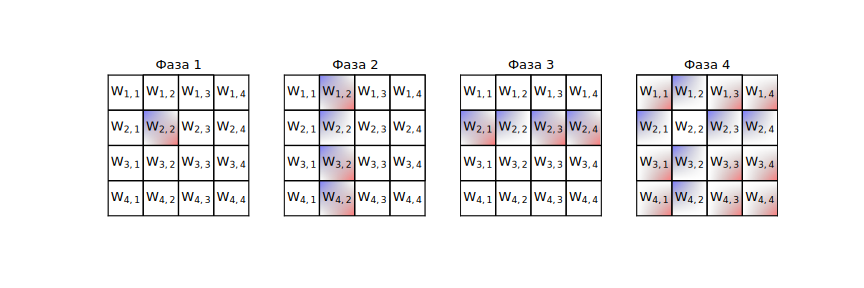
\includegraphics[width=1\textwidth]{images/inf_dep.pdf}
	\caption{Фазы блочного алгоритма Флойда для 2-й итерации}
	\label{img:inf_dep}
\end{figure}

Следует отметить, что в случае, если $p$ не кратно $b$, на краях матрицы появятся неравномерные прямоугольные блоки, тем не менее --- они обрабатываются аналогично основным.

Для параллельных вычислений будет использована собственная реализация пул потоков. В простейшем случае пул состоит из фиксированного числа рабочих потоков. Когда у программы появляется какая-то работа, она вызывает функцию, которая помещает эту работу в очередь. Рабочий поток забирает работу из очереди, выполняет указанную в ней задачу, после чего проверяет, есть ли в очереди другие работы.~\cite[с.~383]{book:threadpool}

Для работы пула потоков необходима система сообщений между потоками (в частности - для оповещения потоков о появлении новой задачи, а также об опустошении очереди задач). Для осуществления этого используется переменная условия. Для корректной работы с переменной условия также используется мьютекс.

\section*{Вывод}

В данной части были приведены ключевые определения, связанные с орграфом, и способ его представления, а также определения примитивов, необходимых для организацией параллельной работы программы. Помимо этого было приведено задание на лабораторную работу и описаны основы последовательного и параллельного алгоритмов, необходимых для его выполнения.

\clearpage
